\chapter{Kyphoplasty}

\section*{Overview}
Kyphoplasty is a procedure used to stabilize a painful vertebral compression fracture. A clinician inserts a small balloon into the collapsed part of the vertebra, inflates it to create a space, removes it, and injects bone cement into that space. The procedure may restore some vertebral height, but this is not guaranteed. Pain relief varies, and the evidence and recommendations for vertebral augmentation differ among clinical guidelines.


\begin{center}
\begin{minipage}{\textwidth}\centering
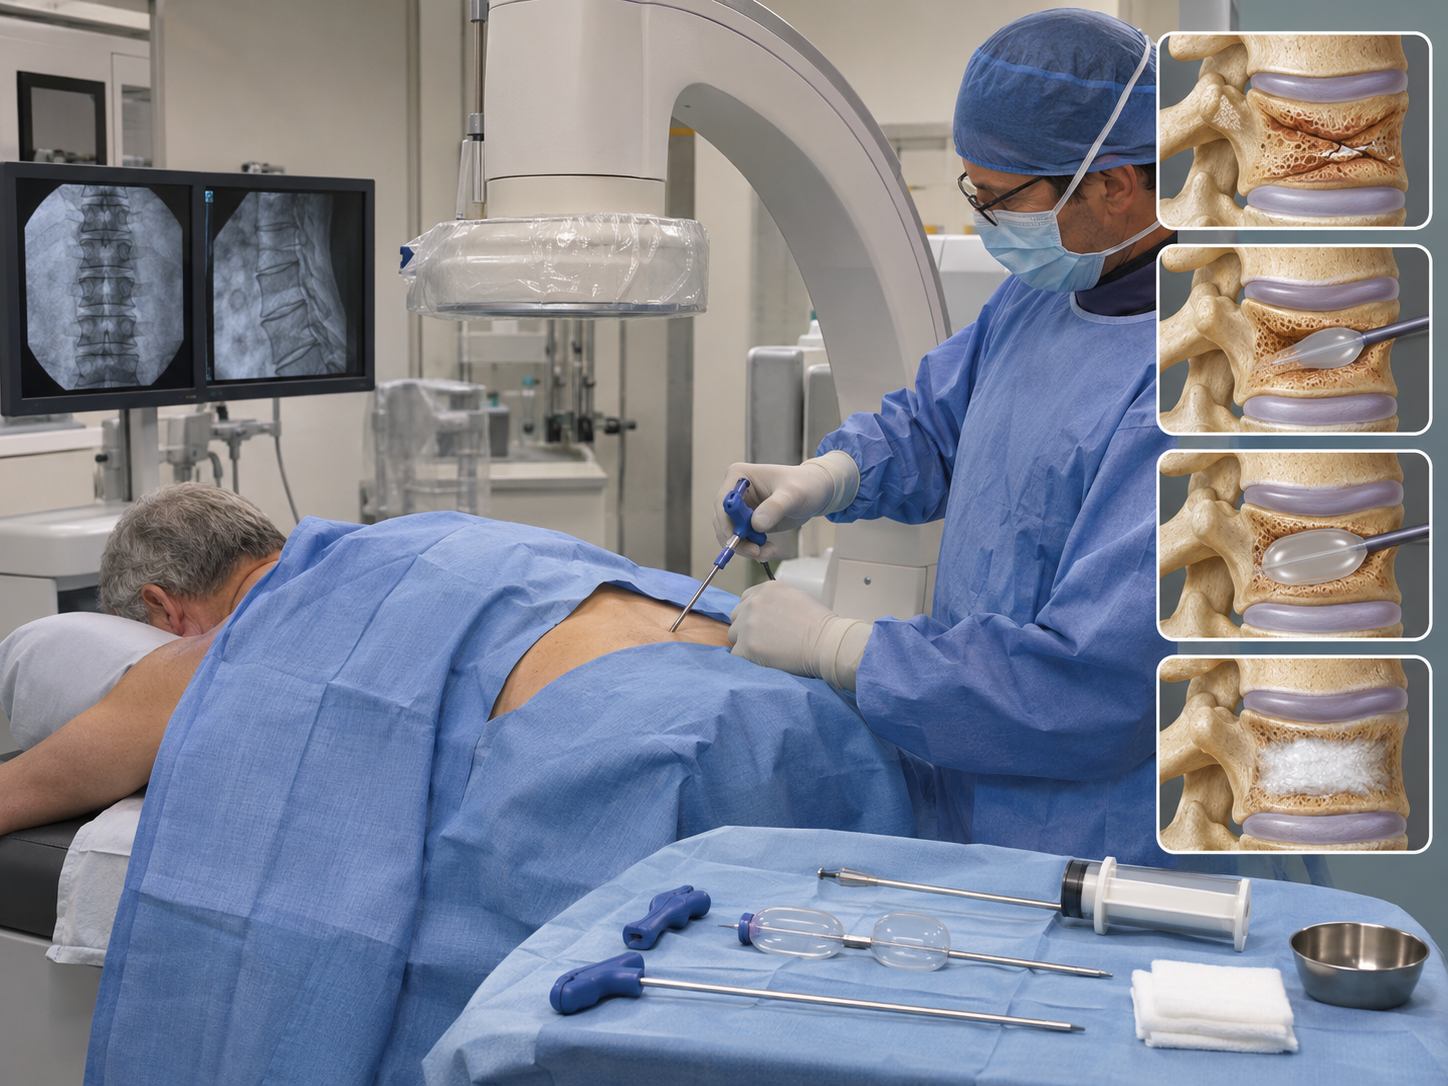
\includegraphics[width=0.82\textwidth]{images/chapters/procedure_kyphoplasty_overview.png}
\captionof{figure}{Kyphoplasty: A surgical team treats a spinal compression fracture; insets show the vertebra and balloon.}
\end{minipage}
\end{center}
\section*{Common Instruments and Equipment}
The exact setup varies by technique and setting. Common items may include:
\begin{itemize}[nosep,leftmargin=*]
  \item vertebral access needles and working cannulas
  \item balloon tamp and bone-cement delivery system
  \item fluoroscopy and monitoring equipment
\end{itemize}

\section*{Alternative Names}
Balloon kyphoplasty; balloon kyphoplasty for vertebral compression fracture; vertebral augmentation

\section*{Principle}
The balloon creates a cavity within the fractured vertebral body. The balloon is removed and bone cement, usually polymethylmethacrylate (PMMA), is injected to stabilize the fracture. Cement hardens quickly. Unlike vertebroplasty, kyphoplasty uses a balloon before cement injection; neither procedure repairs osteoporosis or prevents all future fractures.

\section*{Why It Is Done}
Kyphoplasty may be considered for a recent, unhealed osteoporotic vertebral fracture that causes severe, persistent pain despite appropriate nonsurgical treatment, when examination and imaging show that the pain comes from that fracture. MRI can help identify a recent fracture that is still active; other imaging may be used when MRI is not suitable. The team also considers the person's mobility, overall health, fracture shape, and treatment goals. Usual care for many compression fractures includes appropriate pain relief, safe mobilization, and treatment of underlying osteoporosis. Some guidelines support augmentation for carefully selected patients, while others do not recommend its routine use because trial results have not shown consistent benefit.

\section*{Is This a Primary or Secondary Test or Procedure}
This is an interventional treatment, not a diagnostic test. It is an option for selected patients rather than a routine first treatment for every vertebral compression fracture. It does not treat spinal cord or nerve compression; new neurologic symptoms require assessment for other treatment, which may include surgery.

\section*{How It Is Performed}
The patient is positioned, usually face down, and imaging is used to guide the instruments. Depending on the person's health and the facility, the procedure may use local anesthetic with sedation or general anesthesia. Through one or two small skin incisions, the clinician guides a needle into the fractured vertebra, advances the balloon, and inflates it under imaging. The balloon is deflated and removed, then cement is injected into the space. Imaging is used to check cement placement. The approach and number of vertebrae treated depend on the fracture and the patient's anatomy.

\section*{Preparation}
The team reviews the imaging, fracture timing, pain location, medicines, allergies, bleeding risk, infection symptoms, and relevant heart or lung conditions. Tell the clinician about blood thinners, antiplatelet medicines, prior spine surgery, cancer, fever, or new weakness or numbness. Do not stop blood-thinning medicines without a plan from the clinicians managing them. Fasting instructions depend on whether sedation or general anesthesia is planned. Blood tests or other preparation may be needed based on the person's health.

\section*{Contraindications}
Kyphoplasty is generally not appropriate for an asymptomatic or healed fracture, or when the pain is not clearly linked to the fracture. Active infection, an uncorrected bleeding problem, or medical conditions that make anesthesia unsafe may prevent or delay the procedure.

\section*{Precautions}
A fracture with significant spinal canal narrowing, nerve or spinal cord compression, severe vertebral collapse, or unusual anatomy requires specialist assessment because balloon and cement placement may be unsafe or ineffective. The clinician checks for other causes of back pain and discusses nonsurgical options and the uncertainty of benefit.

\section*{Risks}
Temporary soreness or pain at the needle site can occur. Cement may leak outside the vertebra; this is often seen on imaging without causing symptoms, but rarely can press on a nerve or the spinal cord or enter a blood vessel and affect the lungs. Other uncommon complications include bleeding, infection, nerve injury, fracture of a nearby bone, and complications from sedation or anesthesia. A new fracture in a nearby vertebra can occur after treatment, although it is not always clear whether the procedure increases this risk or whether it reflects the underlying osteoporosis. Severe complications are uncommon but can require urgent treatment.

\section*{Aftercare and Recovery}
After the procedure, staff monitor the patient until stable and check the skin puncture sites and neurologic status. Many patients go home the same day, but some need longer observation. The clinician provides instructions for activity, wound care, pain relief, and when to restart medicines. Mild soreness may last for several days. Some people notice improvement in pain soon after the procedure, but this is not guaranteed; continue prescribed nonsurgical care unless the clinician changes the plan.

\section*{Outcome and Results}
The procedure may stabilize the treated vertebra, but it may not restore normal height, correct spinal curvature, or eliminate pain. Persistent pain may have another cause or indicate another fracture.

\section*{Expected Results}
The goal is to reduce pain and help the person move more comfortably by stabilizing a recent fracture. Some patients improve substantially, while others have little benefit. Any height restoration is usually partial and does not mean that the vertebra has returned to normal.

\section*{Follow-up}
Attend the follow-up visit and discuss whether pain and function are improving. Ask about osteoporosis evaluation and treatment, calcium and vitamin D needs, fall prevention, and other fracture-prevention measures. Kyphoplasty does not treat the underlying bone weakness, and a person may remain at risk for additional fractures.

\section*{When to Seek Medical Care}
Seek urgent care for new leg weakness, numbness, difficulty walking, loss of bladder or bowel control, severe or rapidly worsening back pain, fever, or redness, swelling, or drainage at the puncture site. Sudden shortness of breath, chest pain, fainting, or coughing up blood after the procedure needs emergency assessment.

\section*{References}
\begin{enumerate}
  \item National Institute for Health and Care Excellence (NICE). Percutaneous vertebroplasty and percutaneous balloon kyphoplasty for treating osteoporotic vertebral compression fractures (TA279). \url{https://www.nice.org.uk/guidance/ta279} (accessed November 23, 2026).
  \item National Osteoporosis Guideline Group (NOGG). UK Clinical Guideline for the Prevention and Treatment of Osteoporosis: Section 8, Management of symptomatic osteoporotic vertebral fractures. 2024. \url{https://www.nogg.org.uk/full-guideline/section-8-management-symptomatic-osteoporotic-vertebral-fractures} (accessed November 23, 2026).
  \item American College of Radiology. ACR Appropriateness Criteria: Management of Vertebral Compression Fractures. 2022 update. \url{https://doi.org/10.1016/j.jacr.2023.02.015} (accessed November 23, 2026).
  \item British Orthopaedic Association. Vertebral augmentation for painful osteoporotic vertebral fractures. Evidence-Based Interventions. \url{https://ebi.aomrc.org.uk/interventions/vertebral-augmentation-for-painful-osteoporotic-vertebral-fractures/} (accessed November 23, 2026).
\end{enumerate}

\clearpage
